% Intended LaTeX compiler: pdflatex
\documentclass[11pt]{article}
\usepackage[utf8]{inputenc}
\usepackage[T1]{fontenc}
\usepackage{graphicx}
\usepackage{longtable}
\usepackage{wrapfig}
\usepackage{rotating}
\usepackage[normalem]{ulem}
\usepackage{amsmath}
\usepackage{amssymb}
\usepackage{capt-of}
\usepackage{hyperref}
\author{Construção de compiladores I}
\date{}
\title{Parsing Expression Grammars}
\hypersetup{
 pdfauthor={Construção de compiladores I},
 pdftitle={Parsing Expression Grammars},
 pdfkeywords={},
 pdfsubject={},
 pdfcreator={Emacs 28.2 (Org mode 9.7)}, 
 pdflang={English}}
\begin{document}

\maketitle
\section*{Objetivos}
\label{sec:org7e89929}

\subsection*{Objetivos}
\label{sec:orgbf22bb0}

\begin{itemize}
\item Apresentar o formalismo de Parsing Expression Grammars (PEGs).

\item Apresentar a sintaxe, semântica e boa-formação de PEGs.
\end{itemize}
\subsection*{Objetivos}
\label{sec:org5684def}

\begin{itemize}
\item Apresentar um sistema de tipos para PEGs.

\item Apresentar uma implementação de PEGs em Haskell.
\end{itemize}
\section*{Introdução}
\label{sec:org23d03f7}

\subsection*{Introdução}
\label{sec:org33fa66a}

\begin{itemize}
\item Gramáticas livres de contexto são o \textbf{padrão} para especificar linguagens.

\item Problemas: \textbf{ambiguidade}
\end{itemize}
\subsection*{Introdução}
\label{sec:org6e0895e}

\begin{itemize}
\item Apesar de existirem artifícios para eliminar problemas de ambiguidade, no geral este é um problema \textbf{indecidível}.
\end{itemize}
\subsection*{Introdução}
\label{sec:org9721304}

\begin{itemize}
\item GLCs são um formalismo \textbf{gerativo}, isto é, gramáticas geram palavras.

\item Usamos GLCs para especificar \textbf{reconhecedores}.
\end{itemize}
\subsection*{Introdução}
\label{sec:org03fb404}

\begin{itemize}
\item Essa diferença parece mínima mas é fundamental!
\end{itemize}
\subsection*{Introdução}
\label{sec:org78e706f}

\begin{itemize}
\item Para entender a diferença, vamos considerar a linguagem de palavras com uma quantidade par de zeros.
\end{itemize}
\subsection*{Introdução}
\label{sec:orge85322b}

\begin{itemize}
\item Especificação baseada em geração.
\begin{itemize}
\item Palavras são construídas acrescentando um número finito de 00.
\end{itemize}
\end{itemize}

\(\{s \in 0^{*}\,|\, \exists n \in \mathbb{N}. s = (00)^n\}\)
\subsection*{Introdução}
\label{sec:org502a072}

\begin{itemize}
\item Especificação baseada em reconhecimento
\begin{itemize}
\item Palavras são aceitas se tem tamanho par.
\end{itemize}
\end{itemize}

\(\{s \in 0^{*}\,|\,|s|\mathtt{ mod } 2 = 0\}\)
\subsection*{Introdução}
\label{sec:org66776d4}

\begin{itemize}
\item Uma alternativa recente são as chamadas Parsing Expression Grammars (PEGs).

\item Permitem a especificação de \textbf{reconhecedores}.
\end{itemize}
\subsection*{Introdução}
\label{sec:orgccdf590}

\begin{itemize}
\item Vantagem: não temos mais o problema de ambiguidade.

\item Expressividade: PEGs podem expressar linguagens sensíveis ao contexto.
\end{itemize}
\section*{Parsing Expression Grammars}
\label{sec:orgba4fedc}

\subsection*{Parsing Expression Grammars}
\label{sec:org0e7ad38}

\begin{itemize}
\item Uma PEG G = (V, \(\Sigma\), R, e) é tal que:
\begin{itemize}
\item V: conjunto de não terminais da gramática.
\item \(\Sigma\): alfabeto.
\item R: função total que associa uma \emph{parsing expression} a cada não terminal.
\item e: expressão inicial da gramática.
\end{itemize}
\end{itemize}
\subsection*{Parsing Expression Grammars}
\label{sec:org214889d}

\begin{itemize}
\item Sintaxe de expressões
\end{itemize}

\begin{array}{lcl}
e & \to  & \lambda\,|\, a \in \Sigma \,|\, A \in V\\
  & \mid & e\:e\,|\,e\,/\, e\,|\,e^{*}\,|\,!\,e\\
\end{array}
\subsection*{Parsing Expression Grammars}
\label{sec:orgdcac9a7}

\begin{itemize}
\item Qual o significado de uma parsing expression?

\item Definido em termos de uma relação \(\Rightarrow_{G}\), em que \(G = (V,\Sigma, R, e)\).
\end{itemize}
\subsection*{Parsing Expression Grammars}
\label{sec:orgf816778}

\begin{itemize}
\item Relação \((e,s) \Rightarrow (s_p, s_s)\) denota:
\begin{itemize}
\item Expressão \(e\) processa o prefixo \(s_p\) de \(s\), deixando o sufixo \(s_s\).
\item Caso exista um erro de parsing, utilizamos o símbolo \(\bot\).
\end{itemize}
\end{itemize}
\subsection*{Parsing Expression Grammars}
\label{sec:org3c80f0e}

\begin{itemize}
\item Regra para \(e = \lambda\)
\end{itemize}


\begin{center}
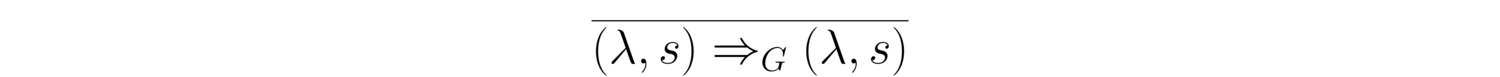
\includegraphics[width=.9\linewidth]{./imgs/image1.png}
\end{center}
\subsection*{Parsing Expression Grammars}
\label{sec:org1e54092}

\begin{itemize}
\item Regras para \(e = a\)
\end{itemize}


\begin{center}
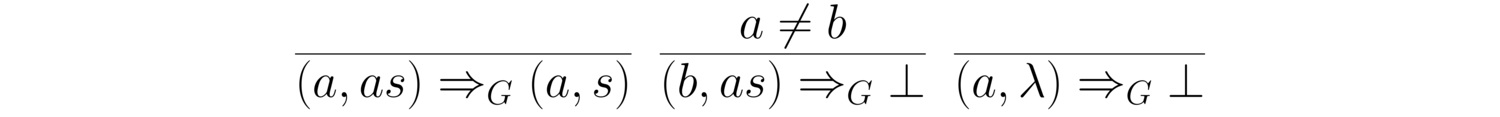
\includegraphics[width=.9\linewidth]{./imgs/image2.png}
\end{center}
\subsection*{Parsing Expression Grammars}
\label{sec:orgcf90cf5}

\begin{itemize}
\item Regras para \(e = A\)
\end{itemize}


\begin{center}
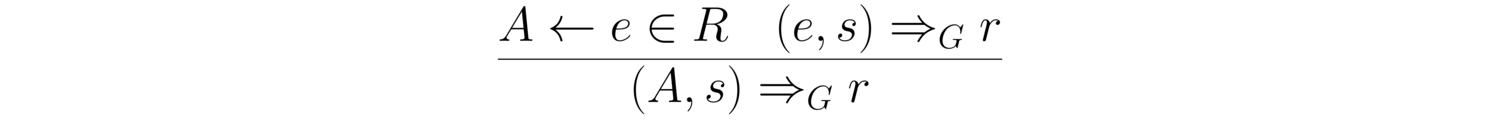
\includegraphics[width=.9\linewidth]{./imgs/image3.png}
\end{center}
\subsection*{Parsing Expression Grammars}
\label{sec:orgb7a1746}

\begin{itemize}
\item Regras para \(e = e_1\:e_2\)
\end{itemize}


\begin{center}
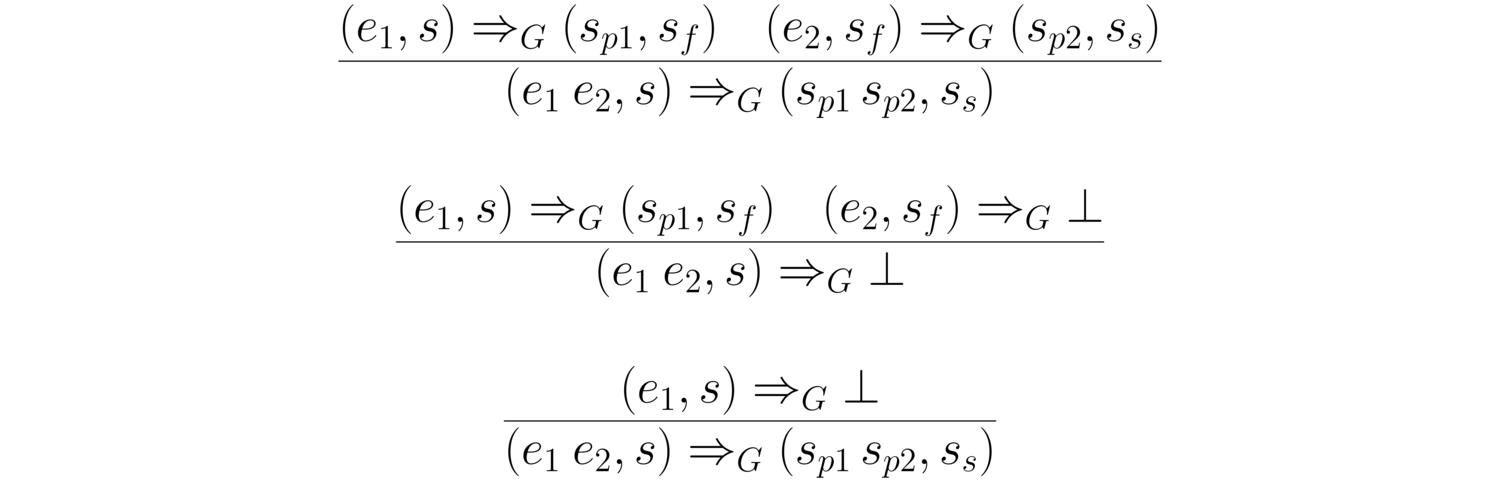
\includegraphics[width=.9\linewidth]{./imgs/image4.png}
\end{center}
\subsection*{Parsing Expression Grammars}
\label{sec:orgf1b30f0}

\begin{itemize}
\item Regras para \(e = e_1\,/\,e_2\)
\end{itemize}


\begin{center}
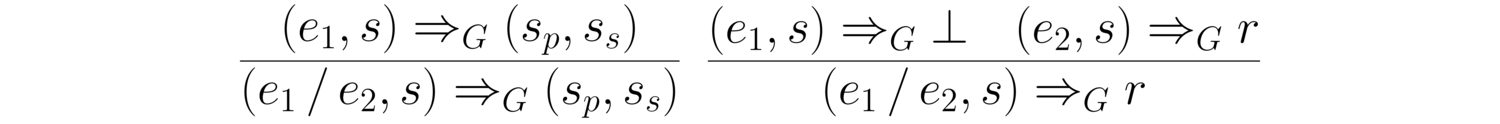
\includegraphics[width=.9\linewidth]{./imgs/image5.png}
\end{center}
\subsection*{Parsing Expression Grammars}
\label{sec:org83293e0}

\begin{itemize}
\item Regras para \(e = e_1^{*}\)
\end{itemize}


\begin{center}
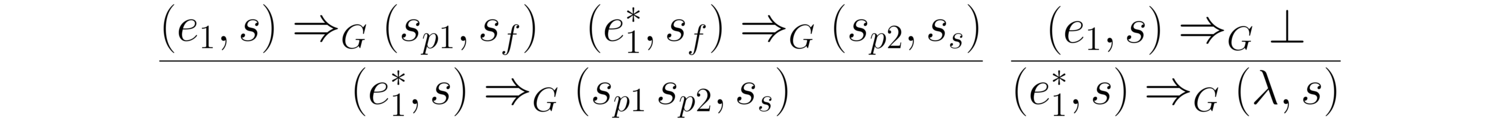
\includegraphics[width=.9\linewidth]{./imgs/image6.png}
\end{center}
\subsection*{Parsing Expression Grammars}
\label{sec:org6eb0187}

\begin{itemize}
\item Regras para \(e = !\,e_1\)
\end{itemize}


\begin{center}
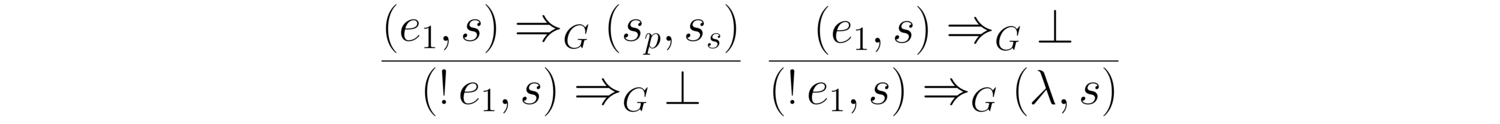
\includegraphics[width=.9\linewidth]{./imgs/image7.png}
\end{center}
\subsection*{Parsing Expression Grammars}
\label{sec:orgd5c17e2}

\begin{itemize}
\item Exemplo
\end{itemize}

\begin{array}{lcl}
A & \leftarrow & a A b \,/\, ab\\
\end{array}

\begin{itemize}
\item Expressão inicial: \(A /\:!\, (a\, /\, b)\: /\: \lambda\)

\item Exemplos da semântica: aabb, a, \(\lambda\)
\end{itemize}
\subsection*{Parsing Expression Grammars}
\label{sec:org6bd0882}

\begin{itemize}
\item Qual o problema com a seguinte gramática?
\begin{itemize}
\item Expressão inicial: A
\end{itemize}
\end{itemize}

\begin{array}{lcl}
A & \leftarrow & A a\,/\,a
\end{array}
\subsection*{Parsing Expression Grammars}
\label{sec:orgbfa8686}

\begin{itemize}
\item Qual o problema com a seguinte expressão?
\begin{itemize}
\item \((a^*)^*\)
\end{itemize}
\end{itemize}
\subsection*{Parsing Expression Grammars}
\label{sec:org1c48c26}

\begin{itemize}
\item Assim como programas em geral, PEGs podem entrar em \textbf{loop}.

\item Basicamente, PEGs são especificações de parsers descendentes recursivos.
\end{itemize}
\section*{Terminação em PEGs}
\label{sec:org8e23bdd}

\subsection*{Terminação em PEGs}
\label{sec:orgc4a3a71}

\begin{itemize}
\item Dizemos que uma expressão \(e\) sucede com uma string \(s\) se:
\begin{itemize}
\item \(\exists s_p\,s_s . (e,s)\Rightarrow_{G} (s_p,s_s)\)
\end{itemize}
\end{itemize}
\subsection*{Terminação em PEGs}
\label{sec:org7a22b09}

\begin{itemize}
\item Relação \(e \rightharpoonup o\), \(o\in\{0,1,f\}\).
\begin{itemize}
\item Caso \(s_p = \lambda\), temos que \(e \rightharpoonup 0\).
\item Caso \(s_p = ay\), temos que \(e \rightharpoonup 1\).
\item Em caso de falha, temos que \(e\rightharpoonup f\).
\end{itemize}
\end{itemize}
\subsection*{Terminação em PEGs}
\label{sec:org396b2d9}

\begin{itemize}
\item Dizemos que uma expressão é bem formada se:
\begin{itemize}
\item Não possui recursão à esquerda direta / indireta.
\item Não é da forma \(e^*\), em que \(e\rightharpoonup 0\).
\end{itemize}
\end{itemize}
\subsection*{Terminação em PEGs}
\label{sec:org30c56a5}

\begin{itemize}
\item Uma PEG é \textbf{bem formada} se todas as suas subexpressões são bem formadas.
\end{itemize}
\subsection*{Terminação em PEGs}
\label{sec:orgf4b0410}

\begin{itemize}
\item Definição original de boa formação é feita em dois passos:
\begin{itemize}
\item Primeiro, define-se quando uma expressão é bem formada.
\item Depois, computa-se o ponto fixo do conjunto de expressões bem formadas de uma gramática.
\end{itemize}
\end{itemize}
\subsection*{Terminação em PEGs}
\label{sec:org0c10bdc}

\begin{itemize}
\item Problemas
\begin{itemize}
\item Definição não composicional
\item Difícil compreensão.
\end{itemize}

\item Solução: Uso de tipos.
\begin{itemize}
\item Falaremos sobre isso quando estudarmos análise semântica.
\end{itemize}
\end{itemize}
\section*{Implementação}
\label{sec:org8d69cb3}

\subsection*{Implementação}
\label{sec:org4cb1ad6}

\begin{itemize}
\item Vamos apresentar uma implementação de PEGs usando combinadores.

\item Note que nossa implementação não irá garantir a terminação!
\begin{itemize}
\item Problema de pesquisa em aberto!
\end{itemize}
\end{itemize}
\subsection*{Implementação}
\label{sec:org2e19bf4}

\begin{itemize}
\item Representando o resultado de uma expressão
\end{itemize}

\begin{verbatim}
data Result s a
  = Pure a           -- did not consume anything. We can backtrack.
  | Commit s a       -- remaining input and result.
  | Fail String Bool -- true if consume any input
  deriving (Show, Functor)
\end{verbatim}
\subsection*{Implementação}
\label{sec:orgcda2a02}

\begin{itemize}
\item Definindo uma expressão.
\end{itemize}

\begin{verbatim}
newtype PExp s a
  = PExp {
      runPExp :: s -> Result s a
    } deriving Functor
\end{verbatim}
\subsection*{Implementação}
\label{sec:org0a96994}

\begin{itemize}
\item Representando a entrada
\end{itemize}

\begin{verbatim}
class Stream a where
  anyChar :: PExp a Char

instance Stream String where
  anyChar = PExp $ \ d ->
    case d of
      (x : xs) -> Commit xs x
      []       -> Fail "eof" False
\end{verbatim}
\subsection*{Implementação}
\label{sec:orgfdc2657}

\begin{itemize}
\item Expressões são applicatives
\end{itemize}

\begin{verbatim}
instance Applicative (PExp s) where
  pure x = PExp $ \ _ -> Pure x
  (PExp efun) <*> (PExp earg)
    = PExp $ \ d ->
        case efun d of
          Pure f   -> f <$> earg d
          Fail s c -> Fail s c
          Commit d' f ->
            case earg d' of
              Pure a -> Commit d' (f a)
              Fail s' _ -> Fail s' True
              Commit d'' a -> Commit d'' (f a)
\end{verbatim}
\subsection*{Implementação}
\label{sec:orgdb97817}

\begin{itemize}
\item Expressões são alternatives
\end{itemize}

\begin{verbatim}
instance Alternative (PExp d) where
  (PExp e1) <|> (PExp e2) = PExp $ \ d ->
    case e1 d of
      Fail _ False -> e2 d
      x            -> x
  empty = PExp $ \ _ -> Fail "empty" False
\end{verbatim}
\subsection*{Implementação}
\label{sec:org2e8dd29}

\begin{itemize}
\item Controlando backtracking
\end{itemize}

\begin{verbatim}
try :: PExp d a -> PExp d a
try (PExp m) = PExp $ \ d ->
  case m d of
    Fail s _ -> Fail s False
    x        -> x
\end{verbatim}
\subsection*{Implementação}
\label{sec:orga0c17fb}

\begin{itemize}
\item Escolha ordenada
\end{itemize}

\begin{verbatim}
(</>) :: PExp d a -> PExp d a -> PExp d a
e1 </> e2 = try e1 <|> e2
\end{verbatim}
\subsection*{Implementação}
\label{sec:org5a19b6b}

\begin{itemize}
\item Símbolos e \(\lambda\)
\end{itemize}

\begin{verbatim}
satisfy :: Stream d => (Char -> Bool) -> PExp d Char
satisfy p = do
  x <- anyChar
  x <$ guard (p x)

symbol :: Stream d => Char -> PExp d Char
symbol c = satisfy (c ==)

lambda :: Stream d => a -> PExp d a
lambda v = PExp $ \ d -> Commit d v
\end{verbatim}
\subsection*{Implementação}
\label{sec:org16c132e}

\begin{itemize}
\item Operador star
\end{itemize}

\begin{verbatim}
star :: Stream d => PExp d a -> PExp d [a]
star e1 = PExp $ \ d ->
  case runPExp e1 d of
    Fail _ _ -> Commit d []
    Pure _ -> Fail "Nullable star" False
    Commit d' v ->
      case runPExp (star e1) d' of
        Fail _ _ -> Commit d []
        Commit d'' vs -> Commit d'' (v : vs)
        Pure _ -> Fail "Nullable star" False
\end{verbatim}
\subsection*{Implementação}
\label{sec:orga4b2b5f}

\begin{itemize}
\item Operador not
\end{itemize}

\begin{verbatim}
not :: Stream d => PExp d a -> PExp d ()
not e = PExp $ \ d ->
  case runPExp e d of
    Fail _ _ -> Pure ()
    _        -> Fail "not" True

and :: Stream d => PExp d a -> PExp d ()
and e = not $ not e
\end{verbatim}
\subsection*{Implementação}
\label{sec:org16791e3}

\begin{itemize}
\item Exemplo: \(\{a^nb^n | n \geq 1\}\)
\end{itemize}

\begin{verbatim}
ab1 :: PExp String String
ab1 = (f <$> symbol 'a' <*> ab <*> symbol 'b') </>
      (g <$> symbol 'a' <*> symbol 'b')
  where
    f x s y = x : s ++ [y]
    g x y = [x,y]
\end{verbatim}
\subsection*{Implementação}
\label{sec:org20951c3}

\begin{itemize}
\item Exemplo: \(\{b^nc^n | n \geq 1\}\)
\end{itemize}

\begin{verbatim}
bc1 :: PExp String String
bc1 = (f <$> symbol 'b' <*> bc <*> symbol 'c') </>
      (g <$> symbol 'b' <*> symbol 'c')
  where
    f x s y = x : s ++ [y]
    g x y = [x,y]
\end{verbatim}
\subsection*{Implementação}
\label{sec:org9220d67}

\begin{itemize}
\item Exemplo \(\{a^nb^nc^n | n \geq 1\}\)
\end{itemize}

\begin{verbatim}
abc1 :: PExp String String
abc1 = f <$> and (ab1 *> not b) <*>
             star a             <*>
             and b              <*>
             bc1                <*>
             not anyChar
  where
    a = symbol 'a'
    b = symbol 'b'
    f _ as _ bcs _ = as ++ bcs
\end{verbatim}
\section*{Concluindo}
\label{sec:org50b68d0}

\subsection*{Concluindo}
\label{sec:orgbe3293c}

\begin{itemize}
\item Nesta aula apresentamos uma alternativa às GLCs: PEGs

\item Apresentamos a sintaxe e semântica de PEGs
\begin{itemize}
\item Discutimos o problema de terminação.
\end{itemize}
\end{itemize}
\subsection*{Concluindo}
\label{sec:orgfcb333c}

\begin{itemize}
\item Apresentamos uma implementação de PEGs em Haskell

\item PEGs não são equivalentes a GLCs
\begin{itemize}
\item Não existe PEG para palíndromos
\item Existe PEG para \(\{a^nb^nc^n\,|\,n\geq 1\}\)
\end{itemize}
\end{itemize}
\subsection*{Concluindo}
\label{sec:org9722d98}

\begin{itemize}
\item Próxima aula: análise sintática ascendente.
\end{itemize}
\section*{Exercícios}
\label{sec:org65d5053}

\subsection*{Exercícios}
\label{sec:org0f375c2}

\begin{itemize}
\item Usando a implementação apresentada, construa uma PEG para expressões aritméticas
envolvendo números, variáveis, adição, multiplicação e parêntesis.
\end{itemize}
\end{document}
